% Copyright 2007 by Till Tantau
%
% This file may be distributed and/or modified
%
% 1. under the LaTeX Project Public License and/or
% 2. under the GNU Public License.
%
% See the file doc/licenses/LICENSE for more details.



\documentclass{beamer}
\usepackage{beamerthemecambridge} 	% Define where theme files are located. 

\usepackage{subfig}

%
% DO NOT USE THIS FILE AS A TEMPLATE FOR YOUR OWN TALKS�!!
%
% Use a file in the directory solutions instead.
% They are much better suited.
%


% Setup appearance:

%\usetheme{default}

%\usefonttheme[onlylarge]{structurebold}
%\setbeamerfont*{frametitle}{size=\normalsize,series=\bfseries}
%\setbeamertemplate{navigation symbols}{}

\usetheme{cambridge}

% Standard packages

\usepackage[english]{babel}
\usepackage[latin1]{inputenc}




%\usepackage{times}
%\usepackage[T1]{fontenc}

%\usepackage{fontspec}
%\setsansfont{Myriad Pro}
%\usefonttheme{professionalfonts}

% Setup TikZ

\usepackage{tikz}
\usetikzlibrary{arrows}
\tikzstyle{block}=[draw opacity=0.7,line width=1.4cm]


% Author, Title, etc.
%Redes Generativas Adversarias Para La Segmentaci�n De Nervios Perif�ricos
\title[REDES GENERATIVAS ADVERSARIAS PARA LA SEGMENTACI�N DE NERVIOS PERIF�RICOS] 
{%
	Redes Generativas Adversarias Para La Segmentaci�n De Nervios Perif�ricos%
}
\subtitle{Director: Hern�n Felipe Arias Garc�a, PhD.}

\author[Jim�nez, Rodriguez, Arias]
{
	Andr�s~Jim�nez~Garc�a\inst{1} \and
	Wilson~A.~Rodr�guez~Mosquera\inst{2} 
	%Till~Nierhoff\inst{3} \and
	%Roded~Sharan\inst{4} \and
	%\textcolor{green!50!black}{Till~Tantau}\inst{5}
}

\institute[T�bingen and others]
{
	\inst{1}%
	Universidad del Quind�o, Armenia(Q)
	\and
	\vskip-2mm
	\inst{2}%
	Universidad del Quind�o, Armenia(Q)
	%  \and
	%  \vskip-2mm
	%  \inst{4}%
	%  Tel-Aviv University, Israel
	%  \and
	%  \vskip-2mm
	%  \inst{5}%
	%  Universit�t zu L�beck, Germany
}

\date[Armenia, Quind�o, 2020]
{Universidad del Quind�o, 2020}



% The main document

\begin{document}
	
	
	
	\begin{frame}
		\titlepage
	\end{frame}
	
	
	
	\begin{frame}{Contenido}
		\tableofcontents
	\end{frame}
	
	
	
	\section{Introducci�n}

		\begin{frame}{�Qu� es el bloqueo de nervios y por qu� es importante?}
			\begin{block}{Bloqueo de nervios}
				El bloqueo de nervios es una estrategia utilizada en la anestesiolog�a para el \alert{tratamiento del dolor} en: Operaciones m�dicas, oncolog�a, etapas post operatorias y por otros casos cl�nicos \cite{Perez2011} \cite{AcedoGutierrez2005}.
			\end{block}
		
			\begin{figure}[!htb]
				\centering
				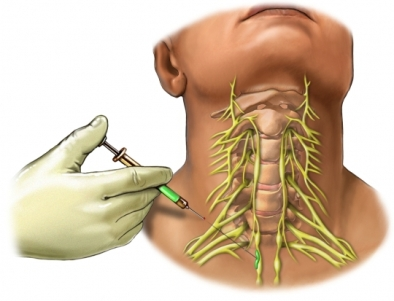
\includegraphics[width=0.35\linewidth]{img/bloqueo}
				\caption{Ilustraci�n de bloqueo para el nervio cervical \cite{bloqueo}.}
			\end{figure}
		\end{frame}
	
		\begin{frame}{Metodolog�as para bloqueo de nervios}
			\begin{figure}[!htb]
				\centering
				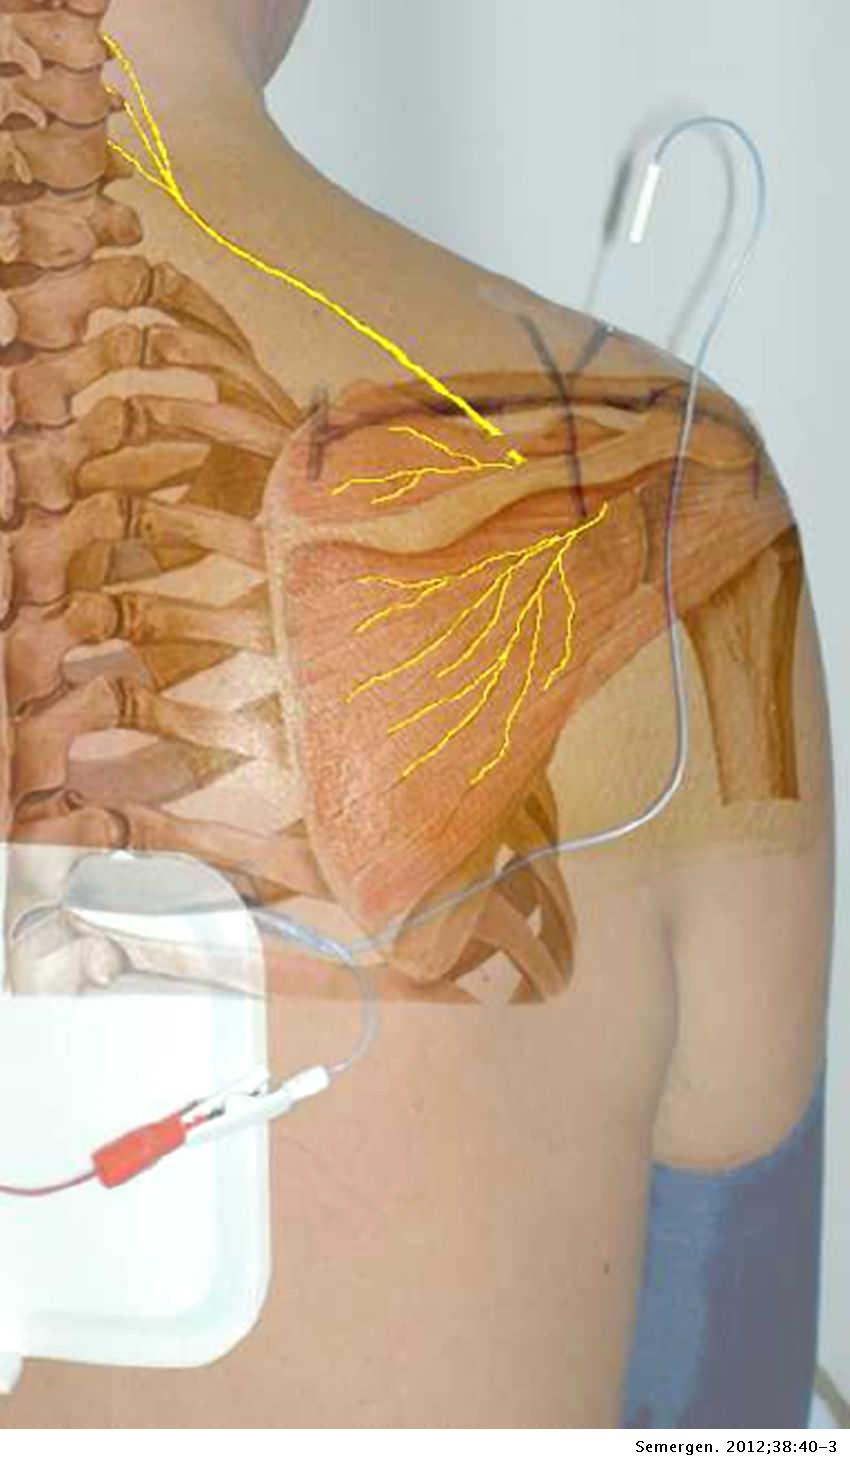
\includegraphics[width=0.25\linewidth]{img/estimulacion}
				\caption{Bloqueo de nervios por medio de \alert{estimulaci�n nerviosa} \cite{estimulacion}}
			\end{figure}
		\end{frame}
	
		\begin{frame}{Metodolog�as para bloqueo de nervios}
			\begin{figure}[!htb]
				\centering
				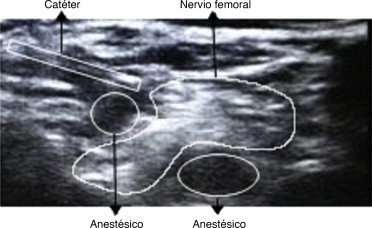
\includegraphics[width=0.7\linewidth]{img/bloqueoUltrasonido}
				\caption{Bloqueo de nervios guiado por \alert{ultrasonido } \cite{bloqueoUltrasonido}}
			\end{figure}
		\end{frame}



	\section{Objetivos}
	
		\begin{frame}{Objetivos}
			\begin{block}{Objetivo General}
				Desarrollar un sistema autom�tico para la segmentaci�n de nervios perif�ricos en im�genes de ultrasonido que permita asistir en su identificaci�n utilizando redes generativas adversarias.
			\end{block}
		\end{frame}
	
		\begin{frame}{Objetivos}
			\begin{block}{Objetivos Especificos}
				\begin{enumerate}
					\item Construir un modelo de aprendizaje generativo adversario que permita generar un mapa de segmentaci�n a partir de una imagen de ultrasonido cuantificando su exactitud por medio de funciones de perdida. 
					\item Desarrollar una estrategia de ajuste que utilice enfoques generativos adversarios para aprender la variabilidad de las texturas anat�micas.  
					\item Evaluar la exactitud del sistema autom�tico para identificar los nervios perif�ricos mediante m�todos cuantitativos y compararlos con enfoques com�nmente utilizados en el estado del arte.
				\end{enumerate}
			\end{block}
		\end{frame}
	
	\section{Red Generativa Adversaria Condicionada}
	
	\begin{frame}{Red Generativa Adversaria Condicionada}
		\begin{figure}[!htb]
			\centering
			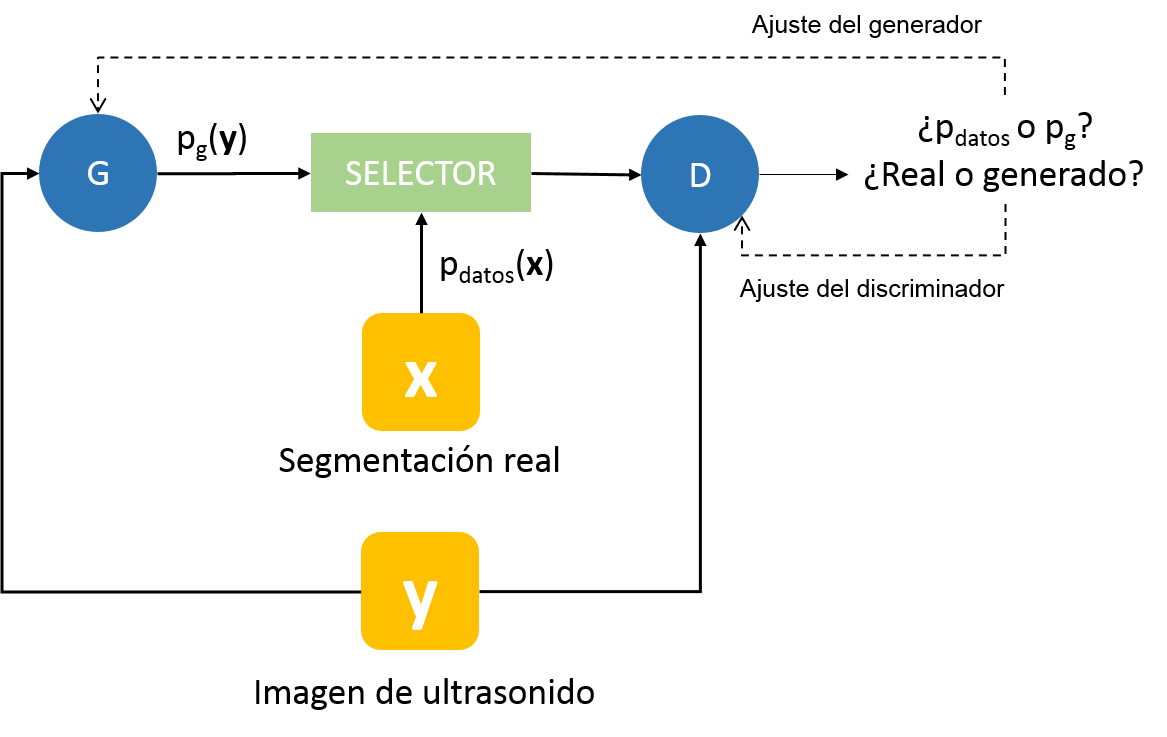
\includegraphics[width=0.7\linewidth]{img/cGANOur}
			\caption{Diagrama de CGAN utilizada para la segmentaci�n de nervios perif�ricos \cite{Isola}}
		\end{figure}
	\end{frame}
	
	\section{Entrenamiento}
	\section{Resultados}
	\section{Conclusiones}
	\section{Trabajos Futuros}
	
	\bibliographystyle{ieeetr}
	\bibliography{bibio}
	
	
\end{document}
